\documentclass{report}
%\usepackage{fullpage}
\usepackage{amssymb}
\usepackage[utf8]{inputenc}
\usepackage{url}
\usepackage{graphicx}

\setlength{\parindent}{0pt}
\addtolength{\parskip}{\baselineskip}

\title{Twitter News Generation - Final Report}

\author{
    \small{Rafał Szymański}\\
  	\and
    \small{Maciek Albin}\\
    \and
    \small{Sam Wong}\\
    \and  
    \small{Suhaib Sarmad}\\
		\and
		\small{Jamal Khan}\\
		\and
		\small{\{rs2909, mja108, sw2309, sss308, jzk09\}@doc.ic.ac.uk}
		\and
		\\Department of Computing - Imperial College London
}



\begin{document} 
	\maketitle
	\tableofcontents
	\newpage

	\chapter{High Level Overview}
	
	Twitter News Generator - An webapp that pairs current events with relevant tweets.

	Traditionally, the media has been presenting news stories biased with the writers’ point of view or agenda. Recruiting readers to join their agendas. This webapp presents a balanced view to the readers. We pair up relevant tweets to news emerging around the world. Our aim is to create a new kind of news reader that also presents the discussion behind the news. 
	
	\section{Product Functionality}

	When a news story breaks, our backend performs a textual analysis on the story to extract keywords. These keywords are then used as the seed to fetch relevant tweets. Once we have a list of relevant tweets, we perform 1) sentiment analysis on these tweets to gauge positivity of each tweet, 2) textual analysis to extract keywords and 3) using 1 and 2 to gauge which tweets should be shown first.

	Once these analyses are done, they are presented in our minimalist yet visually appealing news reading interface. The interface will self-updated periodically, and infinite scroll was implemented to look at past news. Figure~\ref{fig:screen1} shows the final end product.

	\begin{figure}
	 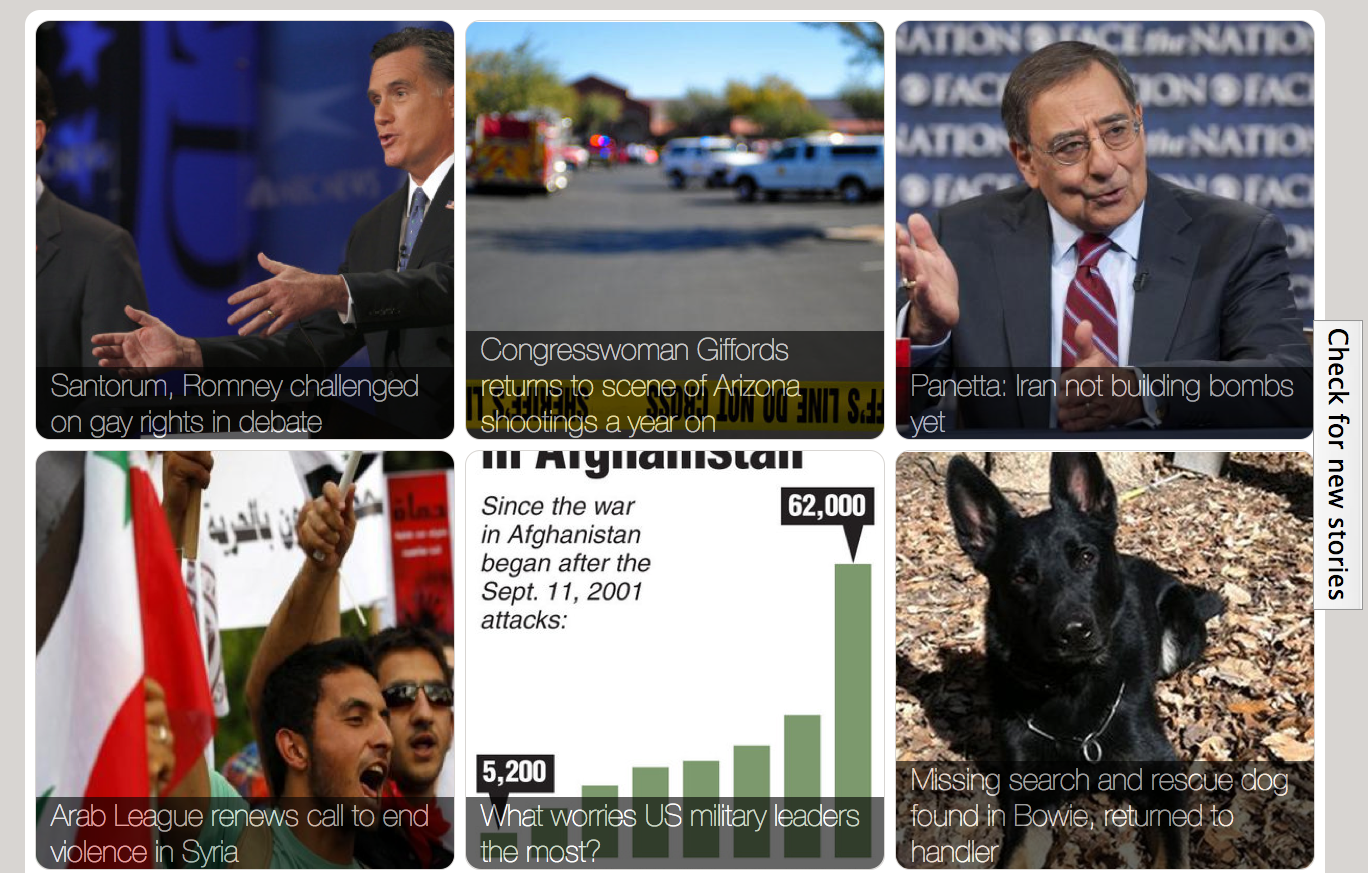
\includegraphics[scale=0.29]{screen1.png}
	 \caption{\label{fig:screen1} Minimalist UI of our end product}
	\end{figure}	
	
	
	\chapter{Technical Overview}
	\begin{figure}
	 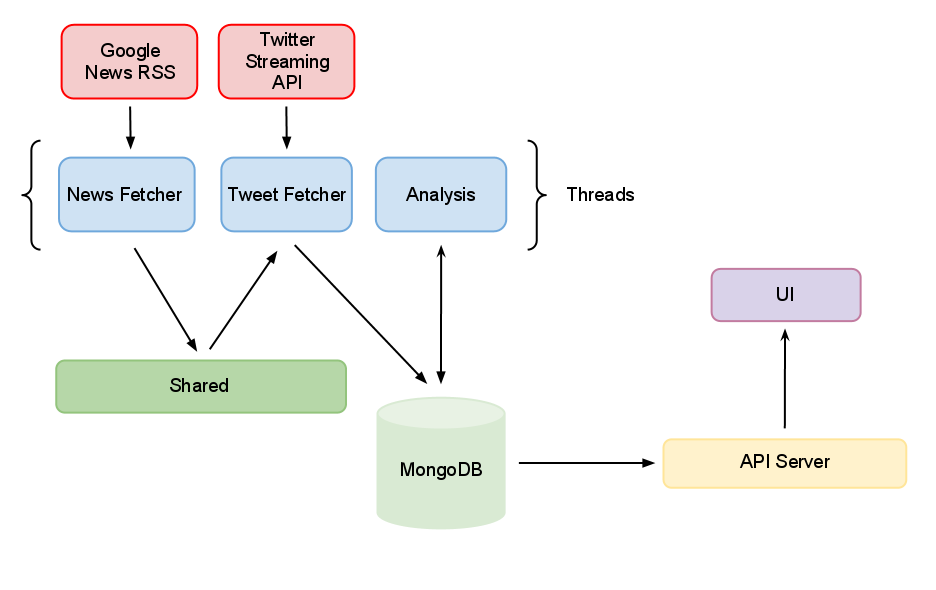
\includegraphics[scale=0.4]{infrastructure.png}
	 \caption{\label{fig:inf_flow} General overview of the information flow in the application. Arrows point into the direction information flows.}
	\end{figure}
	We decided to divide the project into two separate technical parts: \emph{Analysis} and \emph{UI}, that would be connected through our own \emph{API} server\footnote{A general overview of the information flow in the application can be seen in Figure~\ref{fig:inf_flow}.}.
	\begin{description}
	 \item[Analysis] was written in Python and its main tasks were to gather current news, fetch relevant tweets, analyse them in bulk and save the results into a database.
	 \item[API] was also written in Python. It provides easy access to the database for the \emph{UI}.
	 \item[UI] was written in HTML5 and JavaScript. It utilises the API to display the news.
	\end{description}	
	We kept \emph{Analysis} and \emph{UI} as separate as possible. Thanks to that we achieved low coupling and extending the application became quite easy. We use MongoDB as the our database. What follows are short descriptions of how each part of the project works.
	
	\section{Analysis}
	We decided to divide the Analysis process into three separate threads:
	\begin{description}
	 \item[News Fetcher] responsible for fetching current news stories. Getting information relevant to us and generating keywords
	 \item[Tweet Fetcher] responsible for fetching tweets using keywords generated by \emph{News Fetcher}
	 \item[Analysis] uses tweets gathered by \emph{Tweet Fetcher} and info gathered by \emph{News Fetcher} to calculate Twitter's reaction to news stories
	\end{description}
	
	This is the basic sequence of events that happens in the analysis process:
		\begin{enumerate}
		  \item Start three threads: \emph{News Fetcher}, \emph{Tweet Fetcher} and \emph{Analysis}
		  \item \emph{Tweet Fetcher} waits for the \emph{News Fetcher} to get current news
		  \item \emph{News Fetcher} gets current news from the RSS feed
		  \item \emph{News Fetcher} extracts basic information from the RSS feed
		  \item \emph{News Fetcher} generates keywords using AlchemyAPI\footnote{See Chapter~\ref{chap:bib}.}
		  \item \emph{News Fetcher} saves all the info generated into \emph{shared} and goes to sleep for 500s
		  \item \emph{Tweet Fetcher} wakes up gets all the keywords from \emph{shared} and starts fetching tweets mentioning those keywords restarting every time \emph{News Fetcher updates}
		  \item \emph{Analysis} wakes up every 5 minutes and gets current stories from \emph{shared}
		  \item \emph{Analysis} checks if the stories in \emph{shared} are already in DB, if not it inserts them
		  \item \emph{Analysis} gets the tweets saved by \emph{Tweet Fetcher} in last 5 minutes and attaches them to stories in the current period in DB
		  \item \emph{Analysis} performs word cloud generation on the tweets attached to stories
		  \item \emph{Analysis} performs sentiment analysis on the tweets attached to stories using Twitter Sentiment\footnote{See Chapter~\ref{chap:bib}.}
		\end{enumerate}
		
		\section{API}
		API provides a very thin layer between the \emph{UI} and the data stored in the Database. It's written in Python using Flask\footnote{See Chapter~\ref{chap:bib}.} and provides the following calls returning results in JSON:
		\begin{itemize}
		  \item \verb|/api/news| returns the list of 10 current news stories and timestamps for the earliest and the newest stories
		  \item \verb|/api/news/before/<timestamp>| returns a list of 10 news stories before the \verb|<timestamp>| and the timestamp of earliest story
		  \item \verb|/api/news/after/<timest22amp>| returns a list of 10 news stories after the \verb|<timestamp>| and the timestamp of newest story
		  \item \verb|/api/story/<id>| returns a detailed description of the story requested
		\end{itemize}
		
		\section{Server and Production Environment}

		It is essential that all used technologies used be glued together to work on a production environment. For this, on the outer server layer resides Nginx, which proxies requests to the lower level uwsgi process\footnote{This allows Nginx to talk to python and flask} that serves the API and the main page. Static content, such as javascript files or images, are directly handled by Nginx to reduce overhead. Nginx was chosen over the other alternative, Apache, for its lightweight memory footprint, and existing documentation regarding the integration of Nginx, uwsgi, and python.

		Continuous deployment was set up to allow us to code, push a change to the repository, and see it live nearly instantly. Whenever a code push occurs, we have a git post-receive hook that copies the static files appropriately so that they can be served, and restarts the uwsgi process\footnote{This is the process that serves the python code}. This means that as soon as a code push occurs, the new version is live.
		
		
	\chapter{Software Engineering Issues}
	
	\section{Technical challenges, choices and risks}
	What follows is a more detailed description of different parts of the project together with analysis of choices made.
	
	\subsection{Analysis}
		Analysis consists of everything up to and including MongoDB in Figure~\ref{fig:inf_flow}.
		
		\paragraph{Programming Language} We decided to use Python as the main developing language for this part of the project. We needed a relatively lightweight language that would be quite good with connecting to many different web based services and analysing data. Other languages we considered were Ruby and JavaScript (using Node.js).
		
		Most of us had used Node.js before, when working on last years group project. It's a great language for fast and easy realtime communication and it's quite simple to start writing web applications using frameworks like Express\footnote{\url{http;//www.expressjs.com}}. The problem JavaScript had was a lack of threads. We knew we wanted to separate the tweet fetching, news fetching and actual analysis parts out into separate components that could still communicate with each other. It would have been possible with JavaScript by creating 3 different processes, but communication between them would be much more complicated. The other reason we opted out of using Node, was the relative youth of the platform. There just weren't that many useful libraries available.
		
		The choice between Ruby and Python was harder, as they are both fantastic web languages with thriving communities and lots of libraries. It was made easy after doing some more research on analysing twitter and the \emph{social web} in general. We found two great books on the topic\footnote{\emph{Programming Collective Intelligence} and \emph{Mining the Social Web}, for more details see Chapter~\ref{chap:bib}} and both of them advocated using Python for the task. They also came with some tested solutions for fetching tweets and analysing them in bulk, so we decided to use the same language they do.
		
		We are very happy with the choice we've made. Not only have we learned a very popular language but also found lots of help and tools online, which made the project a little bit easier. 
		
		\paragraph{Database} We decided to use MongoDB as our main data store. Most of us had used it before and we were very happy with how it worked. We opted for a NoSQL Document-oriented database, rather than for a classical SQL solution for a couple of reasons.
		
		The data we get for twitter stream is not always the same. Very often there are fields missing, some of them sometimes contain numbers sometimes strings. It would be much harder to save all of that data in a SQL database.
		
		The other advantage MongoDB has here is that it natively operates in JSON, the format twitter data is supplied to us and it makes it extremely easy to save the tweets and retrieve them later.
		
		Our project itself also didn't have a rigid structure initially. We were changing what we write into the database all the time and everything was quite fluid until the very end. The fact that MongoDB didn't impose any structure helped a lot.
		
		\paragraph{Other tools} We decided that in order to attach relevant tweets to news stories we will need to generate keyword relevant to the articles. That turns out to be much trickier than we expected. Keywords need to be specific enough so that the tweets we attach to the story are actually relevant but not so specific that there is no tweets mentioning them. It's quite easy for a person with all the cultural knowledge we have to do that, but writing a program to do that efficiently is actually quite hard.
		
		We initially used TermTopia's TermExtractor\footnote{\url{http://pypi.python.org/pypi/topia.termextract/}}. It was a simple tool that just analysed the title of the article and tried to decide which word in there could be keywords and rank them in order of importance.
		
		We quickly realised that this will not be enough, very often the relevant keywords don't appear in the title, they appear in the text of the news article. We decided to use AlchemyAPI's keyword extractor\footnote{\url{http://alchemyapi.com}}. We emailed them and got special university access that increased the amount of API calls we can make.
		
		We initially wanted to do sentiment analysis ourselves, but we quickly realised it's going to be extremely hard. We did find some interesting papers\footnote{\url{http://www.stanford.edu/~alecmgo/papers/TwitterDistantSupervision09.pdf}}, but realised this approach would involve diving really deep into machine learning and teaching our system to recognise tweets for some time. Fortunately authors of the paper also provide a service for analysing tweet sentiment and an API that goes along with it\footnote{\url{http://twittersentiment.appspot.com/}} and we decided to use that.
		
		\subsection{API}
		From the start we wanted API to be a very thin layer on top of the database. The communication between the API server and the \emph{UI} was supposed to be done using JSON a format that's very easy to use with JavaScript. WE also wanted to keep all of the backend in the same language. It would have allowed possible code migrations from \emph{Analysis} to \emph{API} and vice-versa and also wouldn't require us to learn extra tools.
		
		When looking for a framework we initially considered Django\footnote{\url{http://www.django.org}}, but quickly dismissed it as being way too big for our needs. It requires major setup and is set up for more classic web pages, not live updating, JavaScript based websites.
		
		AFter some research we ended up with two possible choices Bottle\footnote{\url{http://bottlepy.org/docs/dev/}} and Flask\footnote{\url{http://flask.pocoo.org/}}. After quickly going through the documentation it seemed to us that Flask has better support for returning well formed JSON data, so we decided to go with it. API is a relatively small part of the project, so we didn't want to spend too much time making this choice.
		
		\subsection{UI}
		The UI connects to the server's API and displays the information in a clean and appealing tiled layout. Each tile displays an image related to the article aswell as the title of the article in question. On hover/click of a tile, the image folds away (CSS3 eye-candy) revealing a short summary of the article, a word cloud made from common words found in relevant tweets, a list of top relevant tweets and the overall sentiment derived from the relevant tweets.

    We use a HTML frontpage with CSS3 for styling and animations. This allows for a clean and visually appealing user interface. Javascript, JQuery and its various plugins are used to fetch the necessary information from the server API and to make the page dynamic, user friendly and more enjoyable to use.

Specifically we use:
  \begin{itemize}
    \item CSS3 for the fold-away image tile
    \item Javascript/JQuery for fetching news and stories, and adding the news boxes to the page
    \item JQuery Masonry for the dynamic tiled page layout
    \item JQuery WordCloud for on the fly/dynamic word cloud creation
    \item JQuery Infinite Scroll for nice/clever way of getting archived news stories
    \item Various other JQuery plugins for other smaller tasks including nice scrolling
  \end{itemize}
    For article images, we originally wanted to extract the image from the linked article but because we get our news from google which links to several different news sites, writing an extraction method which worked with all these sites proved too difficult and time consuming to be worth it.
    
    Instead we decided to the Google Images API and do an image search with the article's title which almost always resulted in a relevant image. Due to the nature of Google Image search, sometimes the resulting image is too low resolution or the link may be broken. When this occurs, we iterate over the search results until we find an satisfactory image.

    The front page is dynamic, every few minutes it checks with the server if there are any new articles to display and if any changes (tweets/word cloud/sentiment) have occurred to existing articles. It then updates the news tiles accordingly.
    Scrolling to the bottom of the page will invoke a call to fetch past/archived articles. This creates a clean and continuous experience for the user.

    We considered but did not use PHP (or any other server-side scripting language) and opted for Javascript because this relieves some of the workload from the server and also makes it easier to make the page dynamic and update in real time.

    We also considered using SVG and d3.js\footnote{\url{http://mbostock.github.com/d3/}} for rendering additional information such as twitter following/followed networks but due to a design change we decided this was no longer necessary.

		\begin{figure}
  	 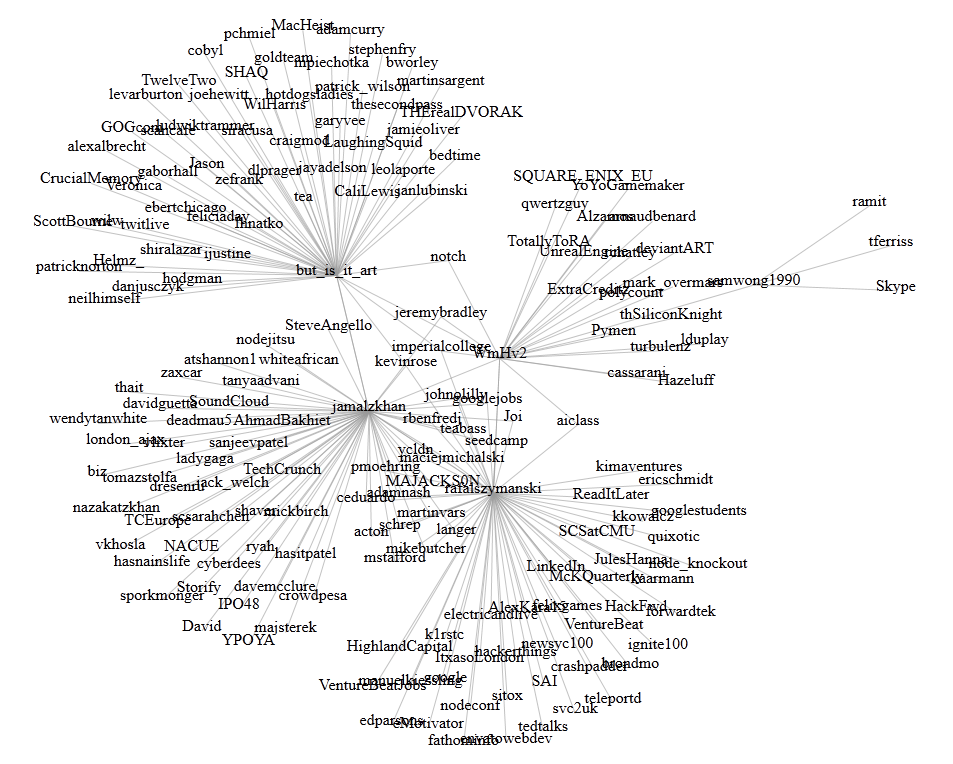
\includegraphics[scale=0.6]{twnet.png}
  	 \caption{\label{fig:twnet} Twitter network created from our group members' accounts using d3.js}
  	\end{figure}
	
		\section{People and Team Management}

		We deem it important to discuss how we have managed our team and worked as a team. As it often happens with group projects, problems relating to group interactions and dynamics surface. Firstly, in our group, everyone knows each other well and is good friends with everyone else, which reduces the authoritative attitude of any one group member towards others. In a real life project, you have a manager with an authoritative position to do things such as lay you off, which certainly induces at least a little bit of motivation. In a university project where all the members are good friends, it is harder to establish an authority that is able to motivate others, especially during a time where everyone has a lot of other personal tasks at hand; motivation has to come from within the group members.

		During this term all of us had lot of other personal responsibilities, including a lot of coursework for other subjects, setting up and studying for internship interviews for next year, and teaching PMT classes, among many others. Considering every one of us has so many personal tasks that directly affect just him and not the group, we saw decreased motivation towards the project from all group members. We have experienced \emph{Social Loafing}\footnote{\url{http://en.wikipedia.org/wiki/Social_loafing}}, which is ``the phenomenon of people exerting less effort to achieve a goal when they work in a group than when they work alone.'' We have had problems keeping to the iteration task assignment on Trello\footnote{\url{http://trello.com}}, ie were not, as individuals, completing the iteration subtasks within the timeline. The root cause of this was likely related to the above explained \emph{social loathing}, and diffusion of responsibility within a group without a clear authoritative figure.

		Our proposed solution was rationalising to all group members the relative importance of this project compared to all other coursework - $440/1700$ points. Receiving a \textbf{C} for our first report was disappointing and a blow to our motivation, as none of us had gotten a C in Imperial before, but on the other hand it was a sign we need increase the quality of our work and approach the project more seriously. This, combined with a meeting with Robert Chatley to discuss problems with report number 1, ensured grades of A+, and A, for reports 2 and 3 respectively. 
		
		Even though over the course of the project, we, as a team, have improved in terms of teamwork, there is still a lot to be improved. We see three important features that we lacked, but that would characterize a more efficient team. Firstly, it is necessary to have an authoritative figure which will watch over the group and assign tasks. It is important that task assignment is followed by the team members. Of course, all topics should be open to a reasonable debate, but in the event progress stalls, the authoritative figure is there to take a decision and lead the project forward. Secondly, it would be beneficial if, when working on the project, the team members looked at each other as co-workers and not simply as school friends. If everyone is good friends outside of the project, it is necessary to introduce a change in attitude, so that, while remaining friends, team members can work as co-workers towards a common goal - the completion of the project. Without a change in attitude, we risk the teamwork project to be a considered a fun 'game' of not much importance, and the impact of this will be visible on the final output. Thirdly, as said by Peter Drucker\footnote{\emph{"What gets measured, gets managed"}}, we claim that is vital to measure progress frequently. Trello was a big help in establishing who is to do what, but what was lacking was an enforcement of these assignments. We have planned to have frequent scrum meetings regarding the completion of tasks, but instead, since we all saw each other during lectures anyways, we usually discussed the progress without having had a dedicated meeting. This was an unsatisfactory decision - we should have gotten into the habit of having dedicated progress meetings, where everyone has to showcase what they achieved in the previous 2 or 3 days. Under the knowledge that one has to have something to present at a team meeting, there is a much higher chance that said team member will have produced an amount of work worth discussing. Otherwise, with no set meetings, there is less incentive for individuals to contribute fairly and frequently.

		We now discuss the assignment of tasks and group subdivision. We have separated our group of five people as follows: 2 for UI, and 3 for backend, so everyone is doing what they are more comfortable with. From time to time, but maybe not as often as we could have done, both of these subteams utilized pair programming. Many times one of us knew something useful, for example a specific MongoDB query syntax, and can help the other without having to resolve to Google. This ensures a good flow of information between the team, and levels out our knowledge. A visible problem was the following scenario: we are working in the same location, but not currently pair programming. Person $A$ is concentrating and has a train of thought, while person $B$, interrupts to ask for a triviality such as the aforementioned MongoDB query syntax, which one easily find on google within 30 seconds. Now $A$ has lost concentration and needs to get back on their train of thought. We see that $B$ has shortened the amount of work for himself, but has lowered the total productivity and output of the group. This is to be avoided at all costs. There is a time to discuss and ask questions, and there is a time to work quietly. The group most not get itself into a state of perpetual back-and-forth questioning of, for example, API syntax, or else group productivity is greatly diminished. Nevertheless, when we set to do a session of pair programming, output and learning were both increased.
		
		 We discussed that the group was separated into frontend and backend, but we still thrived to have a \emph{bus count}\footnote{\url{bit.ly/j1zquA} - quite interesting article.}\footnote{Bus count - ``how many people in your team have to get hit by a bus before you’re all dead in the water''} of the size of our group - we wanted everyone to understand, and if needed, to work on any part of our stack. In the end, this has not fully materialized, as the frontend group don't know the intricacies involved in the threading of the backend processes, and the backend team is not aware of the various UI hacks the frontend team had to develop to have a nice cross-browser and pretty UI.
		
		
		\section{Collaboration Tools Used}
		
			\subsection{Git}
		
			We have used the git version control system for keeping track of the project, for easily reverting if there is a problem, and for having a very quick deploy mechanism. Whenever a code push occurs to our git repository, we have a git post-receive hook that copies the static files appropriately, and restarts the appropriate processes. This means that as soon as a code push occurs, the new version is live right away.
		
			\subsection{Trello}
		
			Trello\footnote{\url{http://trello.com}} is a very good piece of software by FogCreek. It is a digital board that allows you to create post-its and write the product backlog, and move tasks between the product backlog, the current iteration, and the finished tasks. We have used Trello throughout and found it very useful. See Figure~\ref{fig:trello} to have an overview of how Trello operates.
			
			\begin{figure}
			 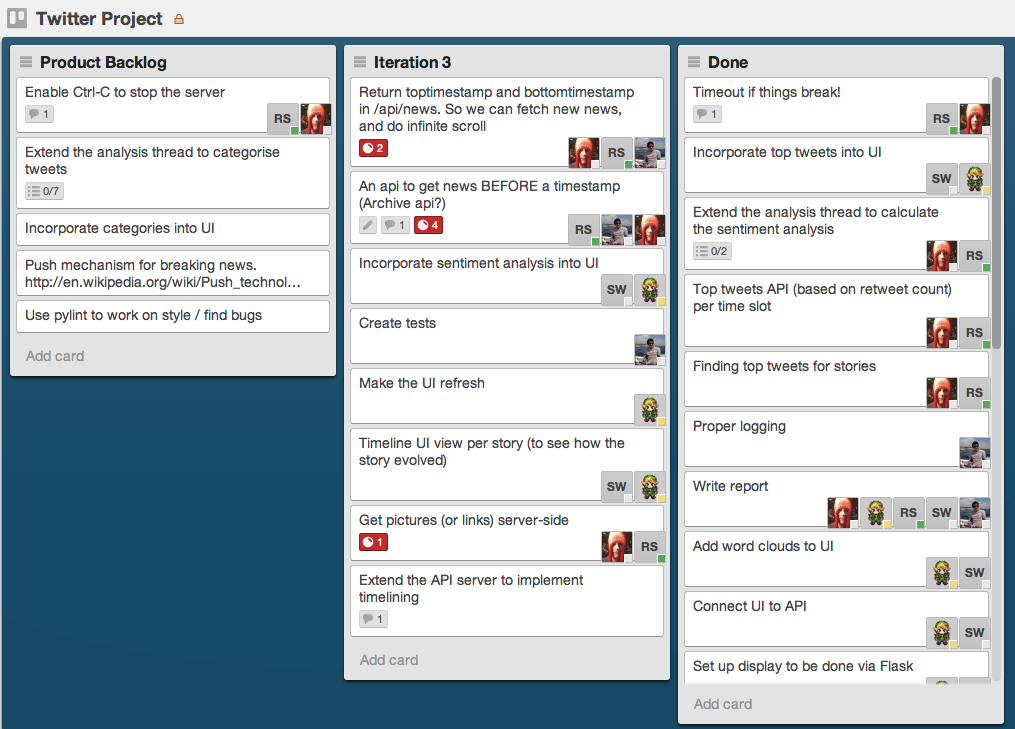
\includegraphics[scale=0.4]{trello.png}
			 \caption{\label{fig:trello} Trello project management board.}
			\end{figure}
		
			\subsection{Skype}
		
			We extensively used Skype to discuss the project and set up team meetings.
			
		\section{Development Techniques}
		
		We adopted agile development methodologies, but as discussed in the section on people management, we have had some problems in having set project meetings. Nevertheless, we have adopted the use of iterations and developed using iterations plans.
		
		\textbf{First iteration of iteration plan}

		\begin{itemize}
			\item First Iteration MVP - basic news augmenting functionality and live updates.
			\begin{itemize}
				\item Setup DB and server to receive Tweets and RSS
				\item Research suitable DB (MongoDB) – Select frameworks and architecture – digging into twitter API and RSS
				\item Design algorithms to generate keywords (Look into using natural language processing libraries, there are a lot available for Python)
				\item UI Mockups and UX Research
				\item UI Implementation: Framework and plugins to use (eg jQuery, jQuery plugins, Twitter Bootstrap, etc)
				\item Getting the web app hosted
			\end{itemize}
			
			\item Second Iteration
			\begin{itemize}
				\item Polished and Efficient implementation including Debugging, refactoring and optimisation
			\end{itemize}
			
			\item Third Iteration
			\begin{itemize}
				\item Extensions including: • Sentiment Analysis algorithm • Categorization algorithm 
			\end{itemize}
			
			\item Fourth Iteration
			\begin{itemize}
				\item Final Product
			\end{itemize}
			
		\end{itemize}
		
		After submitting our first report we realised the Iteration plan we proposed was flawed. In many parts instead of focusing on the user facing features we have reported on the technical aspects of what we will do. One whole iteration was dedicated to “Debugging, refactoring and optimisation”. 

		Therefore, we drafted a new iteration plan and described what the project goals are in terms of user-facing features.
		
		\textbf{Second iteration of iteration plan}
		
		\begin{itemize}
			\item First Iteration
			\begin{itemize}
				\item Setup DB and server to receive Tweets and RSS
				\item Research suitable DB (MongoDB) – Select frameworks and architecture – digging into twitter API and RSS
				\item First attempt at the UI. It will be polished and new features will be added throughout iterations.
				\item Generate keywords from news stories and fetch relevant tweets. This is a necessary part of the entire system.
				\item Display current news stories
				\item Getting the web app hosted
			\end{itemize}
			
			\item Second Iteration
			\begin{itemize}
				\item Wordclouds generated from tweets related to news stories.
				\item Influential tweets related to news stories.
			\end{itemize}
			
			\item Third Iteration
			\begin{itemize}
				\item Add the ability to analyse whether the tweets are positive or negative and present the aggregated result in the UI.
			\end{itemize}
			
			\item Fourth Iteration
			\begin{itemize}
				\item Categorise tweets and based on these categories categorise the news stories themselves. Add that to UI.
			\end{itemize}
			
			\item Fifth Iteration
			\begin{itemize}
				\item Fetch pictures relevant to news stories and present them in the UI.
			\end{itemize}
			
			\item Sixth Iteration
			\begin{itemize}
				\item Final application polish and validating if everything is really really working before final submission.
			\end{itemize}
			
		\end{itemize}
		
		We were satisfied with this plan. We skipped Iteration 4 because we thought it doesn’t align with our project aim, but apart from that, we followed the plan and made accountable progress along the way.
	
			\section{Testing}
			  Testing our project was challenging. Since it is more of a real-time system that just analyses data we did not have any models to test. Nevertheless we needed a way to check if the program is working correctly.

			  \subsection{Unit and Mock Testing}

			  We used the PyUnit\footnote{\url{http://pyunit.sourceforge.net/}} module for incorporating unit tests in our code. An example of where we used this was in the RSS thread where we were testing functionality of all the functions written for this module. For this we had to create a mock rss fetcher object and run tests on it.

			  Having said this, it was very difficult to test some parts of the system as there is a lack of clear models, for example having unit tests for keyword generation or tweet fetching is difficult to implement as they use external APIs.

			  \subsection{Logging and Debugging}

			  Instead of using standard print statements to output the state of our system, which is composed of the RSS, Analysis and Twitter Thread, we incorporated a flexible event logging system.\\
			We are able to leave our system and if an error occurs we can trace exactly which thread caused it and at which point in the program as opposed to the usual debugging.
		  The logger was also incorporated so that we have different levels of importance in logging i.e. have logging for general information of what is going on in the system and logging for errors. We are also able to log messages to different output sinks including the console and files.

				\begin{figure}
				 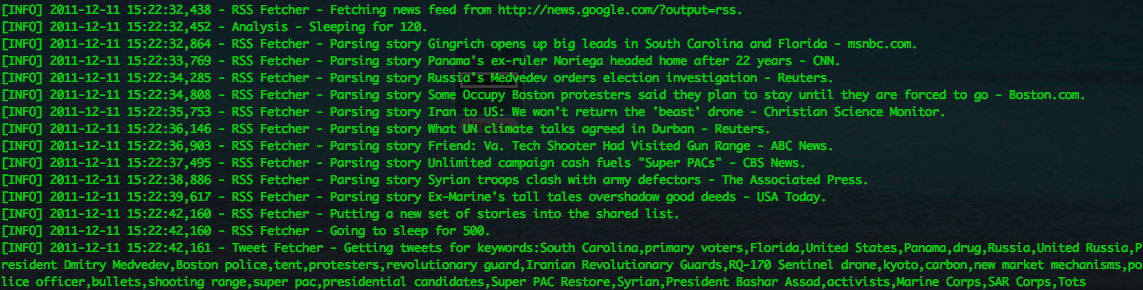
\includegraphics[scale=0.32]{logger.png}
				 \caption{\label{fig:logger} Customised logger.}
				\end{figure}
				
		   \subsection{Unit and Mock Testing}

		  	  We used the PyUnit\footnote{\url{http://pyunit.sourceforge.net/}} module for incorporating unit tests in our code. An example of where we used this was in the RSS thread where we were testing functionality of all the functions written for this module. For this we had to create a mock rss fetcher object and ran tests on it.

				\subsection{UI Testing}
				To debug the UI, Google Chrome’s Developer tools and Firebug were used. These tools were used to inspect the requests the UI issued, the network activities, debug layout and monitor performance.
	
		\section{Summary of each members contribution}
		
				We have tried to establish fair contribution by everyone by assigning to everyone tasks on Trello, and believe that it has worked well and ensured a rather fair individual contribution. As stated beforehand, we had a clear distinction between the people working on the frontend and backend.
		
		  \subsection{Maciek Albin}
		    \begin{tabular}{l | p{10cm} r}
		     \emph{\large Date} & \emph{\large Comments} & \emph{\large Hours}\\
		     \hline
		     12/10/2011 & Advanced network generation for follower/folowee relations. & 3\\
		     20/10/2011 & More work on the network generation. & 4\\
		     28/10/2011 & Initial internal API definition and basic implementation. & 2\\
		     28/10/2011 & Fixes to inter thread communication. & 2\\
		     02/11/2011 & Refactoring. & 3\\
		     02/11/2011 & Implemented keyword generation using Alchemy API. & 2\\
		     03/11/2011 & Implemented basic analysis thread. & 4\\
		     04/11/2011 & Assigning tweets to stories in analysis thread. & 3\\
		     04/11/2011 & Added short summaries and links to stories DB. & 2\\
		     08/11/2011 & Added wordclouds to the API. & 1\\
		     10/11/2011 & Refactoring. & 3\\
		     30/11/2011 & Fixed bugs in the logger. & 2
		    \end{tabular}

		  \subsection{Jamal Khan}
		  \begin{tabular}{l | p{10cm} r}
	     \emph{\large Date} & \emph{\large Comments} & \emph{\large Hours}\\
	     \hline
		  11/10/2011 & Initial creation of the RSS Fetcher using python module feedparser. & 2\\
	    31/10/2011 & Keyword extraction completed for each story using Alchemy API. & 4\\
	    4/11/2011 & Implemented Flask Server creating API for the front end for the site as well as relevant database calls to fetch stories. & 7\\
	    10/11/2011 & Added functionality of getting stories by timestamp for the API. & 2\\
	    25/11/2011 & Completed flexible logger for each thread, so we can see exactly what is going on. & 7\\
	    12/11/2011 & Unit testing for RSS Fetcher completed. & 4
	  \end{tabular}

	  \subsection{Suhaib Sarmad}
	    \begin{tabular}{l | p{10cm} r}
	     \emph{\large Date} & \emph{\large Comments} & \emph{\large Hours}\\
	     \hline
	     27/10/2011 & Resource research and UI mockup & 4\\
	     28/10/2011 & Basic grid UI proof of concept & 3\\
	     09/11/2011 & Implementation of basic jQuery Masonry (tiled) UI & 2\\
	     10/11/2011 & Create tiles in UI from server news API & 4\\
	     11/11/2011 & CSS/HTML Tile layout, split into title/summary, picture, sentiment, word cloud, tweet list & 5\\
	     11/11/2011 & UI debugging and cross-browser compatibility: works on all tested browsers except IE & 2\\
	     12/11/2011 & Added tweets to tweet list using Twitter REST API and keywords from server API, added custom jQuery scrollbars & 1\\
	     12/11/2011 & Added pictures to tiles using Google Images API and article titles & 2\\
	     12/11/2011 & Generating html5 word cloud from keywords from server API & 3\\
	     19/11/2011 & CSS3 transitions research and testing for big picture UI & 2\\
	     01/12/2011 & Automatic refreshing and fetching of new news articles from server & 4\\
	     09/12/2011 & Sentiment bar prototype & 1
	    \end{tabular}


		  \subsection{Rafał Szymański}
		    \begin{tabular}{l | p{10cm} r}
		     \emph{\large Date} & \emph{\large Comments} & \emph{\large Hours}\\
		     \hline
		     10/10/2011 & Initial commit for the project. Basic implementation in Python of a script that given a keyword  fetches the live streaming API for the given keyword and writes it to the Mongo database. & 6\\
	       11/10/2011 & Bug fixes and a short readme. & 2\\
	       12/10/2011 & Fetching the follower/folowee graph and saving to a file. Basic analysis with NetworkX. & 3\\
	       20/10/2011 & More working on generating the user graph. & 2\\
	       21/10/2011 & Big update. Gets headlines from Google news RSS, generates keywords using Termtopia, sets up twitter stream, saves to Mongo and repeats every 5 minutes. & 7\\
	       01/11/2011 & Improving the threading of the program - added condition variables and fixed previous threading bugs. & 4\\
	       04/11/2011 & Working on instant deployment environment using Flask, Nginx, uwsgi, and a couple other technologies. Took forever to do but afterwards, after every git push, the new version is live straight away. & 10\\
	       07/11/2011 & Improvements to the instant deployment - new git hook, and a control script that allows remote restarting and clearing of the database. & 4\\
	       08/11/2011 & Wordcloud generation. Goes through each tweet, finds the most occurring words and adds that data for each analysis period. & 4\\
	       11/11/2011 & Improvements to control script. & 2\\
	       30/11/2011 & Sentiment analysis for each period. Gets sentiment using an API and adds to Mongo. & 5\\
	       04/12/2011 & Top tweets based on the number of retweets. & 2\\
	       04/12/2011 & Added all my new data to the frontend API. & 2
		    \end{tabular}

		  \subsection{Sam Wong}
		  \begin{tabular}{l | p{10cm} r}
	     \emph{\large Date} & \emph{\large Comments} & \emph{\large Hours}\\
	     \hline
		   12/10/2011 & Python development & 1\\
	     02/11/2011 & UI Prototype 1 & 3\\
	     09/11/2011 & UI Prototype 2 & 4\\
	     20/11/2011 & UI Prototype 3 & 5\\
	     21/11/2011 & UI debugging & 1\\
	     25/11/2011 & UI features experimentation & 1\\
	     01/12/2011 & UI features refinement & 1\\
	     01/12/2011 & Auto-refresh & 2\\
	     01/12/2011 & infinite scroll proof of concept & 3\\
	    \end{tabular}
	
	\section{Ethical and Environmental Impact of our Project}	

	Ethical and environmental impact was a point of discussion in one of the previous reports, and we deem it interesting to add this discussion to this final report. We see the following possible ethical and environmental issues:

	\begin{itemize}

	  \item All technologies that we are using are open source. Python has an OSI-approved license\footnote{\url {http://docs.python.org/license.html}}, our server is written using Flask which is BSD Licenced\footnote{\url{http://flask.pocoo.org/docs/license/}} and MongoDB is also open source\footnote{\url{http://www.mongodb.org/display/DOCS/Licensing}}. The server is the widely used Nginx, which has a BSD-like license.

		\item We are storing tweets, which are not our property. We copy the whole tweet to our database, which originally is the property of the original author and of Twitter. This is not exactly a compromising situation, but it nevertheless should be considered from an ethical standpoint.

		\item We are possibly aggregating information and presenting it in such a fashion that could reveal new and interesting patterns - patterns that might be surprising or ones that others don't agree with. We would also probably need to state that the results are merely the results of our algorithmic analysis, and not our personal viewpoint regarding the current news story.

		\item In addition, the news stories we are aggregating from Google News may be biased as it is based on what Google believes to be the top stories, and other peoples point of view as to what news is top may differ around the world.

		\item Our project currently only works for just top 10 stories from google news, and the volume of tweets is already quite high (can be as high as 50 a second). This means that the database is growing large quite quickly. If this project were to be extended to support many more news services, it would have to be distributed over more machines, along with more database instances to support the larger volume of data. This would be something to consider if machines or EC2 instances were to be bought. Already, after running the product over the night, there was a notification from the VPS provider notifying about high disk IO rate. These type of problems could be classified as an environmental issues.
	\end{itemize}
	
	
	\chapter{Validation and Conclusions}
	
	\section{User Validation}
	
	From time to time we asked for feedback on the user facing products. This was done so that we could make design and functionality choices. We talked to our supervisor Jeremy Bradley, and he liked our user interface but wanted us to add pictures for each news story, we consequently went ahead with this and received very positive feedback.
	
	\section{Code Validation}
	
	We used Pylint4 to validate the Python code which we wrote. This was done to check for errors such as incorrect indentation, bad naming conventions for class names and functions, among others. Checking for errors and validating the UI side of the project was done using the W3 Validator at \url{http://validator.w3.org/}.
	
	\section{Conclusion}
	
	
	
	
	
	\chapter{Bibliography and Tools used}\label{chap:bib}
	
	Taking into account the fact that this wasn't a research project requiring extensive external material, we do not provide a full bibliography, but provide links to sources we have used and consulted when working on this software engineering project.
	
	\begin{itemize}
		\item Backend Resources
		\begin{itemize}
			\item 	\url{http://pyunit.sourceforge.net/} - Unit testing
			\item 	\url{http://nginx.org/} - Backend server
			\item 	\url{http://projects.unbit.it/uwsgi/} - For nginx to speak with python
			\item 	\url{http://alchemyapi.com} - API for keyword extraction
			\item   \url{http://pypi.python.org/pypi/topia.termextract/} TermTopia's TermExtractor
			\item   \url{http://twittersentiment.appspot.com/} Twitter Sentiment Analizer
			\item 	\url{http://mongodb.com} - Data store used 
			\item 	\url{http://www.logilab.org/857} - Pylint
		\end{itemize}
		
		
		\item Frontend Resources
		\begin{itemize}
			\item 	\url{http://validator.w3.org/} - HTML Validator
			\item 	\url{http://jquery.com/} - jQuery
			\item 	\url{http://masonry.desandro.com/} - jQuery Masonry Plugin
		\end{itemize}
		
		\item Other Resources
		\begin{itemize}
			\item 	\url{http://trello.com} - Online task board
			\item 	\url{http://www.python.org/doc/} - Python documentation
			\item 	\url{http://git-scm.com/} - Version control system used
			\item 	\url{https://github.com/} - For storing code + wiki
			\item 	\url{http://flask.pocoo.org/} - Python web framework
			\item 	\url{http://news.google.com/} - News source
			\item 	Programming Collective Intelligence, Toby Segaran, OReilly Media, 2007
			\item 	Mining the Social Web, Matthew A. Russell, OReilly Media, 2011
		\end{itemize}
		
	\end{itemize} 
	
	\chapter{Appendix}
	
	\section{Team Meetings}
	\begin{tabular}{c | l p{7cm} r}
    \emph{\large Date} &  \emph{\large Venue} &  \emph{\large Subject} &  \emph{\large Attended}\\
    \hline
    14/10/2011 & Lab Round Table & Choose which project to do & \(G\)\\
    18/10/2011 & Skypeland & Choose which project to do & \(G\)\\
    21/10/2011 & Lab Round Table & Discovered the original plan is infeasible due to constraints set by Twitter, draft backup plan & \(G\)\\
    27/10/2011 & Lab Round Table & Plan approved, Design Architecture & \(G \smallsetminus \{\texttt{Suhaib}\}\)\\
    3/11/2011 & Lab Round Table & Progress Report (Backend, and UI Prototype I) & \(G \smallsetminus \{\texttt{Rafal}\}\)\\
    10/11/2011 & Lab Round Table & UI Prototype II presentation, API requests and design & \(G \smallsetminus \{\texttt{Maciej}\}\)\\
    17/11/2011 & Lab Round Table & UI Prototype III. Post-JB-meeting discussion & \(G \smallsetminus \{\texttt{Jamal}\}\)\\
    24/11/2011 & Skypeland & Incremental improvements & \(G \smallsetminus \{\texttt{Sam}\}\)\\
    1/12/2011 & Skypeland & Extensions ideas & \(G \smallsetminus \{\texttt{Suhaib}\}\)\\
    8/12/2011 & Skypeland & Features prioritisation & \(G\)\\
  \end{tabular}

  \(G=\{\texttt{Rafal}, \texttt{Sam}, \texttt{Suhaib}, \texttt{Jamal}, \texttt{Maciek}\}\)\\


	

\end{document}
